\chapter[Stability of hybrid vs. vaccine immunity against BA.5 infection over 8 months]{Stability of hybrid versus vaccine immunity against BA.5 infection over 8 months}
\label{chapter:2023-covid19-02}

%%%%%%%%%%%%%%%%%%%%%%%%%%%%%%%%%%%%%%%%%%%%%%%%%%%%%%%%%%%%%%%%%%%%%%%%
\noindent\underline{J. Malato}, R.M. Ribeiro, E. Fernandes, P.P. Leite, P. Casaca, C. Antunes, V.R. Fonseca, M.C. Gomes, and L. Graca. Stability of hybrid versus vaccine immunity against BA.5 infection over 8 months. \textit{The Lancet Infectious Diseases}. 2023; 23(2):148--150. doi: \url{https://doi.org/10.1016/S1473-3099(22)00833-7}.

%%%%%%%%%%%%%%%%%%%%%%%%%%%%%%%%%%%%%%%%%%%%%%%%%%%%%%%%%%%%%%%%%%%%%%%%
% \begin{totheeditor}
% zzz
% \end{totheeditor}

%%%%%%%%%%%%%%%%%%%%%%%%%%%%%%%%%%%%%%%%%%%%%%%%%%%%%%%%%%%%%%%%%%%%%%%%
%%%%%%%%%%%%%%%%%%%%%%%%%%%%%%%%%%%%%%%%%%%%%%%%%%%%%%%%%%%%%%%%%%%%%%%%
%%%%%%%%%%%%%%%%%%%%%%%%%%%%%%%%%%%%%%%%%%%%%%%%%%%%%%%%%%%%%%%%%%%%%%%%
\section{Introduction}

The coverage of SARS-CoV-2 vaccination in large parts of the world, together with the high number of breakthrough infections, especially following the emergence of Omicron subvariants, makes hybrid immunity (resulting from vaccine and infection) common. Hybrid immunity, particularly after BA.1 or BA.2 infection, confers substantial protection against the BA.5 infection \citep{malatoRiskBAInfection2022, altarawneh2022ProtectiveEffect, hansen2023RiskReinfection}. However, although the waning of protection afforded by natural infection in non-vaccinated individuals or by vaccination has been well documented \citep{chemaitelly2021WaningBNT162b2, goldberg2022ProtectionWaning} the stability of hybrid immunity, specifically against the BA.5 subvariant, now dominant in many countries, has not been thoroughly addressed.

We used the Portuguese Covid-19 registry (SINAVE), which includes all notified cases of infection in the country on the basis of an official positive test and irrespective of clinical presentation, to investigate the risk of reinfection with BA.5 in a highly vaccinated population previously infected with BA.1 or BA.2 subvariants. We included the population aged 12 years or older, for whom the vaccination coverage was greater than 98\% at the end of 2021 (additional description in Section~\ref{2023-sec:covid19-02-methods}). The registry is very comprehensive due to legal requirements for compensation payment during mandatory isolation. We include infection data from the start of the pandemic until Sept 14, 2022.

We identified the periods of dominance (over 90\% of the isolates) of BA.1 and BA.2 (Jan 1--Apr 17, 2022) and BA.5 infections (June 1--Sept 14, 2022) using the national SARS-CoV-2 genetic surveillance data and divided those periods into 15 day intervals (Figure~\ref{fig:fig1-stability-hybrid-immunity}A). We then calculated the relative risk (RR) of BA.5 infection in each interval for individuals that had the first infection during each BA.1 and BA.2 dominance subinterval, compared with individuals also vaccinated but without any previous documented infection. Reinfection was defined as two positive tests in the same individual, at least 90 days apart. We found that the RR increased from around 0.06 to around 0.35 between 3 months and 8 months post BA.1 or BA.2 infection (Figure~\ref{fig:fig1-stability-hybrid-immunity}B). Indeed, the RR initially increases rapidly, then more slowly, stabilising at around 0.37.

\begin{figure}
    \centering
    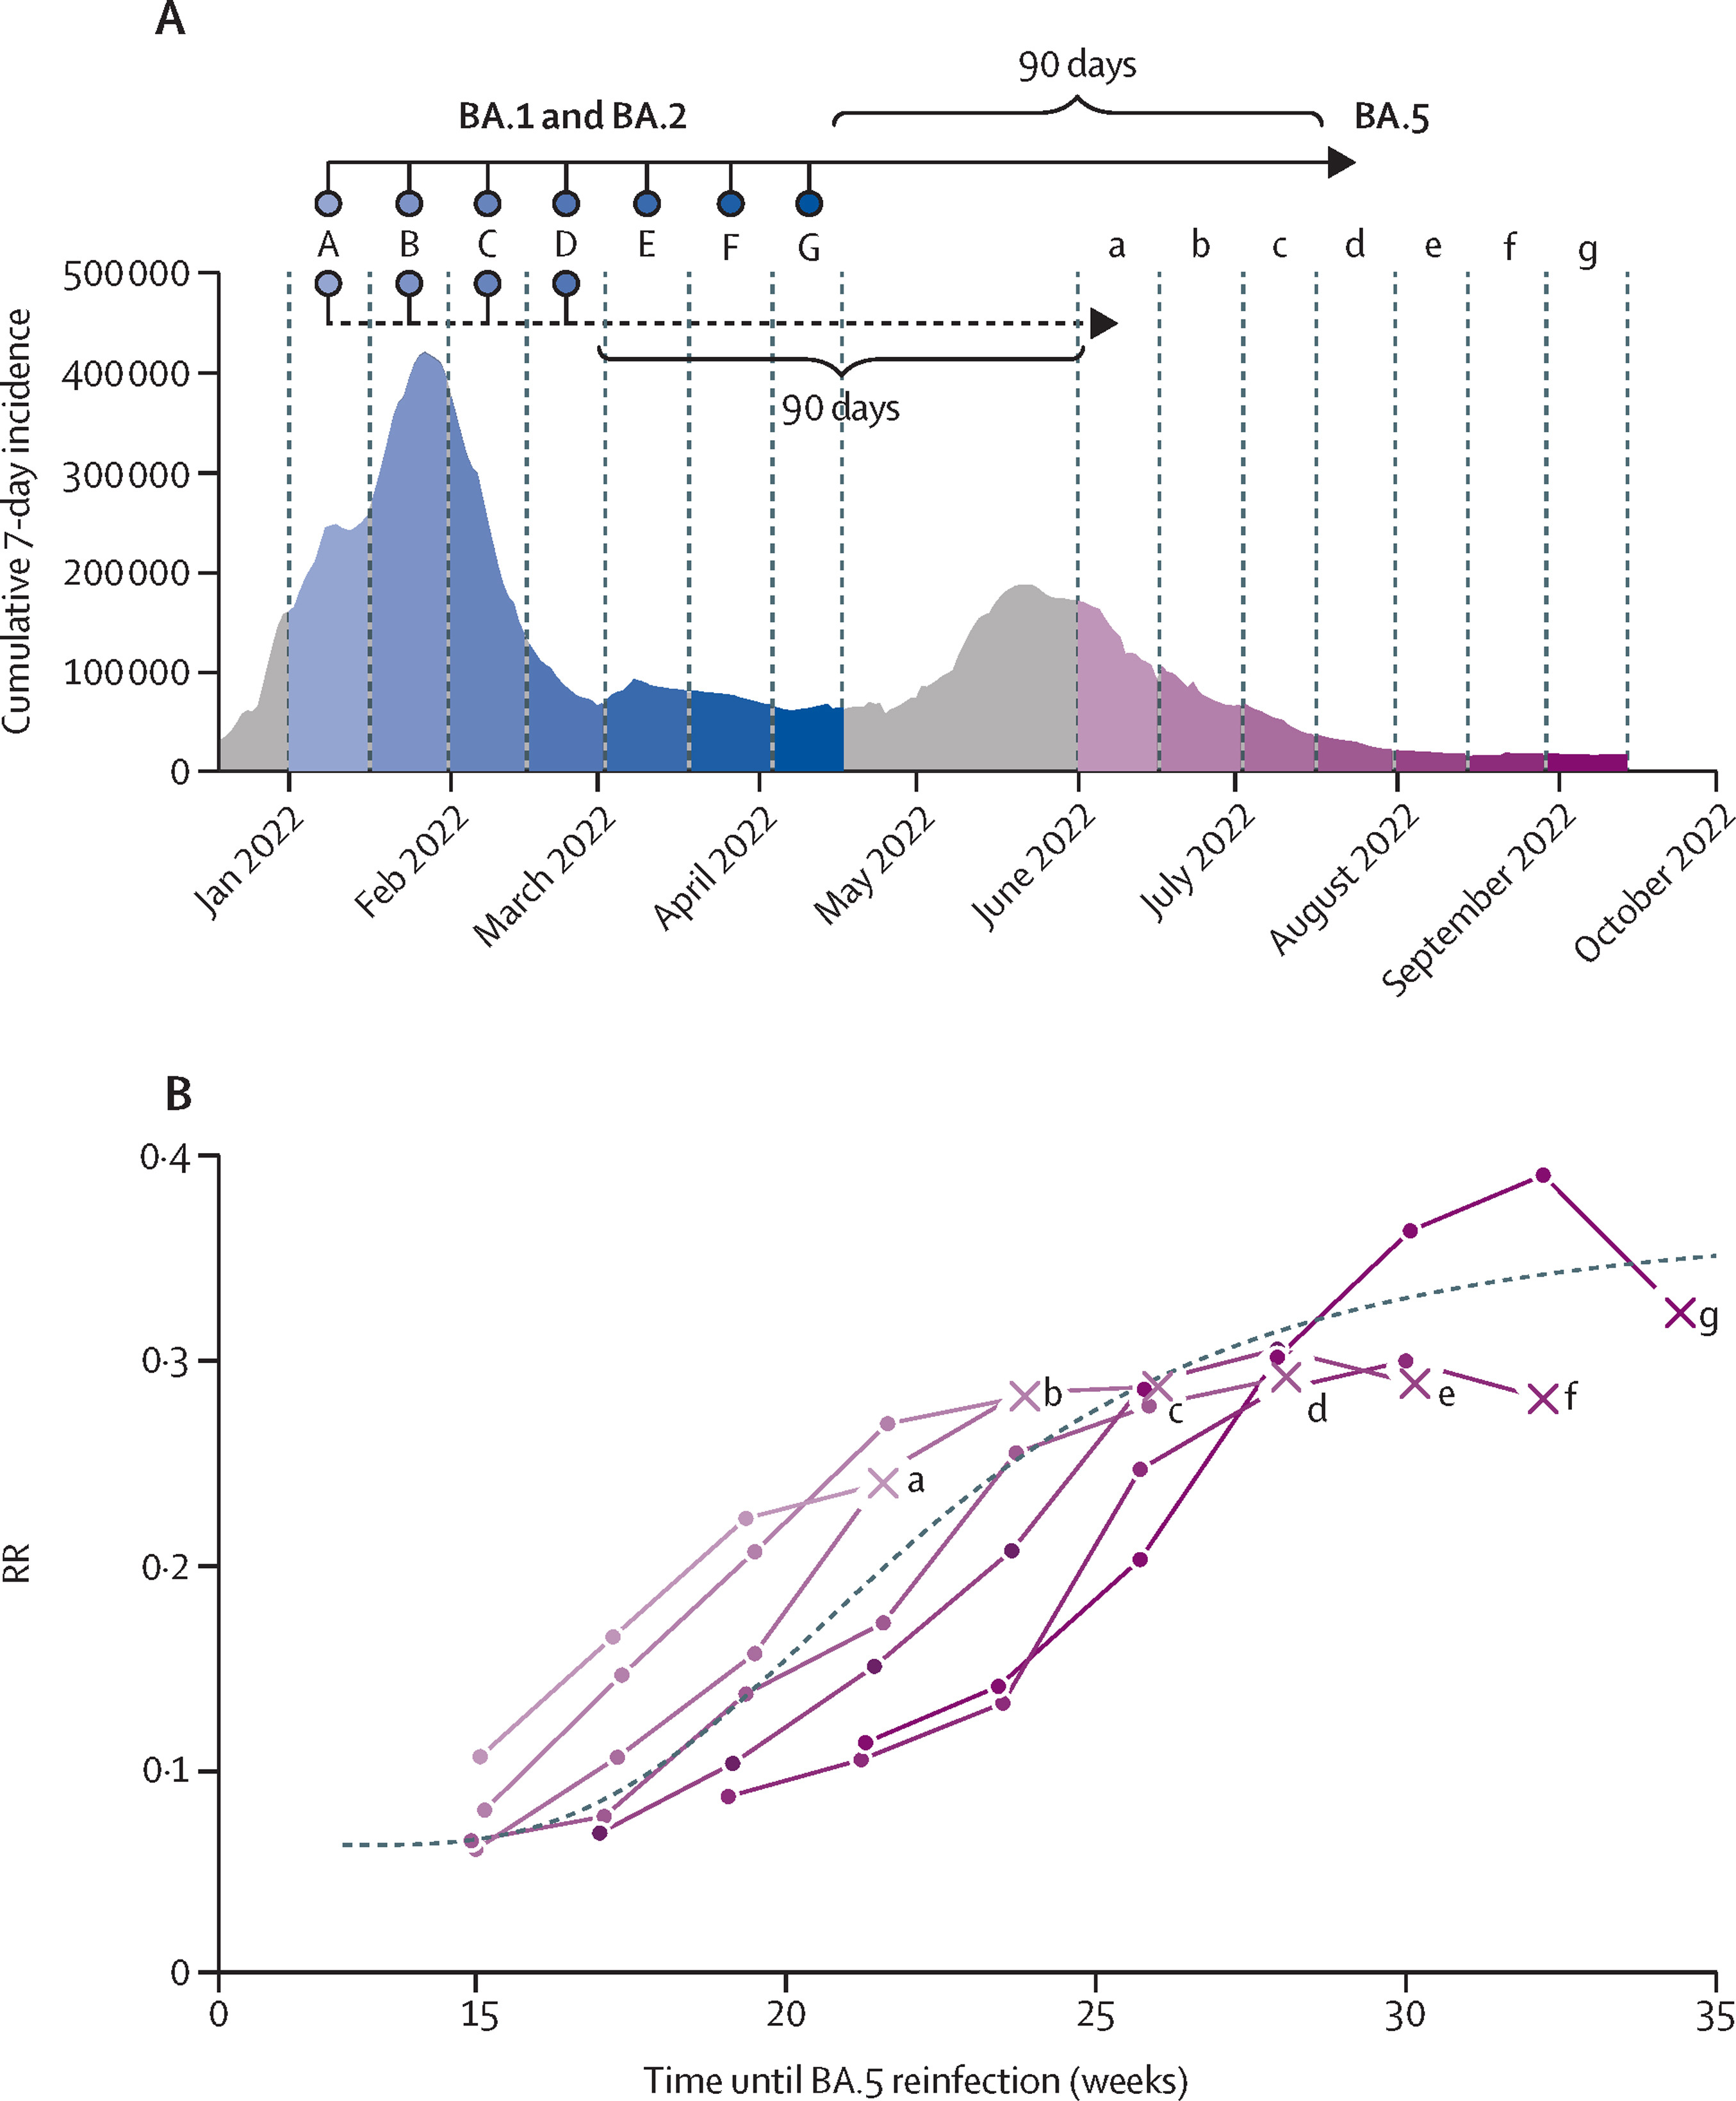
\includegraphics[width=0.8\textwidth]{chapter/2023-covid19-02/figures/fig1-stability-hybrid-immunity}
    \caption[Stability of hybrid immunity protection against BA.5 infection following infection with BA.1 or BA.2 subvariants]{Stability of hybrid immunity protection against BA.5 infection following infection with BA.1 or BA.2 subvariants. (A) Incidence of documented SARS-CoV-2 infection overlaid with the period of dominance of the BA.1 and BA.2 variants, Jan 1--Apr 14, 2022, divided into 15-day sub-intervals (shades of blue), and the period of dominance of the BA.5 variant, Jun 1--Sep 14, 2022, also divided into 15-day sub-intervals (shades of purple). Two illustrative comparisons are represented. In period d (BA.5 dominance), the risk of infection was compared between individuals with a first documented infection in one of the seven subintervals of BA.1 and BA.2 dominance (A--G), represented with the solid arrow. In the second example with the dashed arrow, in period a of BA.5 dominance, the risk of infection was compared between individuals with a first documented infection in the first four periods of BA.1 and BA.2 dominance (A--D), as reinfections were only considered 90 days following the first infection. (B) RR of reinfection versus first infection in each subinterval of the period of BA.5 dominance (curves a--g, corresponding with the periods of the same letter as in (A) over time since the first infection. The increase in risk is well described by a saturating function (Equation~(\ref{eq:omicron-infection-risk})) as represented by the fitted line (dashed, black). RR, relative risk.}
    \label{fig:fig1-stability-hybrid-immunity}
\end{figure}
% Figure 1
% Figure~\ref{fig:fig1-stability-hybrid-immunity}

The present authors previously assessed the effect of unreported infections in the calculation of RR \citep{malatoRiskBAInfection2022}. Here, we mitigate this effect by calculating the RR for the same interval of BA.5 infection for individuals infected by BA.1 or BA.2 in distinct periods, thus with a constant frequency of unreported infections. In any case, our findings are consistent throughout the entire dataset. Our registry-based dataset includes data on essentially the whole population, but only includes data on positive tests. This feature precludes using a test-negative study design, which has been successfully used in other studies of RR \citep{altarawneh2022ProtectiveEffect, ayoub2022EstimatingProtection}. However, previous reports indicate that the estimates of protection efficacy using the national registry are well aligned with studies that used a test-negative design, albeit in a different population \citep{malatoRiskBAInfection2022, altarawneh2022ProtectiveEffect}. Studies since 2021 have made clear the potential for immune imprinting, with one study \citep{chemaitelly2022ProtectionReinfection} suggesting that protection against infection waned after the booster (relative to primary series). In our study, essentially the whole population is vaccinated with the booster dose, and therefore we cannot distinguish effects of booster versus primary series. However, our results of increased protection with hybrid immunity versus vaccine immunity, agrees with the overall conclusion of that study that ``imprinting effects are unlikely to negate the overall public health value of booster vaccinations'' \citep{chemaitelly2022ProtectionReinfection}.

This study shows that hybrid immunity following infection with Omicron BA.1 or BA.2 when compared with vaccine-only immunity leads to substantially increased protection against BA.5 reinfection for up to 8 months.

%%%%%%%%%%%%%%%%%%%%%%%%%%%%%%%%%%%%%%%%%%%%%%%%%%%%%%%%%%%%%%%%%%%%%%%%
%%%%%%%%%%%%%%%%%%%%%%%%%%%%%%%%%%%%%%%%%%%%%%%%%%%%%%%%%%%%%%%%%%%%%%%%
%%%%%%%%%%%%%%%%%%%%%%%%%%%%%%%%%%%%%%%%%%%%%%%%%%%%%%%%%%%%%%%%%%%%%%%%
\section{Methods}
\label{2023-sec:covid19-02-methods}

%%%%%%%%%%%%%%%%%%%%%%%%%%%%%%%%%%%%%%%%%%%%%%%%%%%%%%%%%%%%%%%%%%%%%%%%
\subsection{Participant selection}

We followed an approach similar to what we reported in a previous registry-based study \citep{malatoRiskBAInfection2022}. The population included in the study comprises: (1) All individuals resident in Portugal aged 12 years and older without a documented infection until the start of the follow-up period, which is June 1st to September 14th, 2022; and (2) All individuals resident in Portugal aged 12 years and older with a single documented infection between January 1st, 2022 (the initial period of dominance of BA.1) up to 90 days before the follow-up period and no other previous infection (see flowchart, Figure~\ref{fig:covid19-02-flowchart}).

\begin{figure}[h]
    \centering
    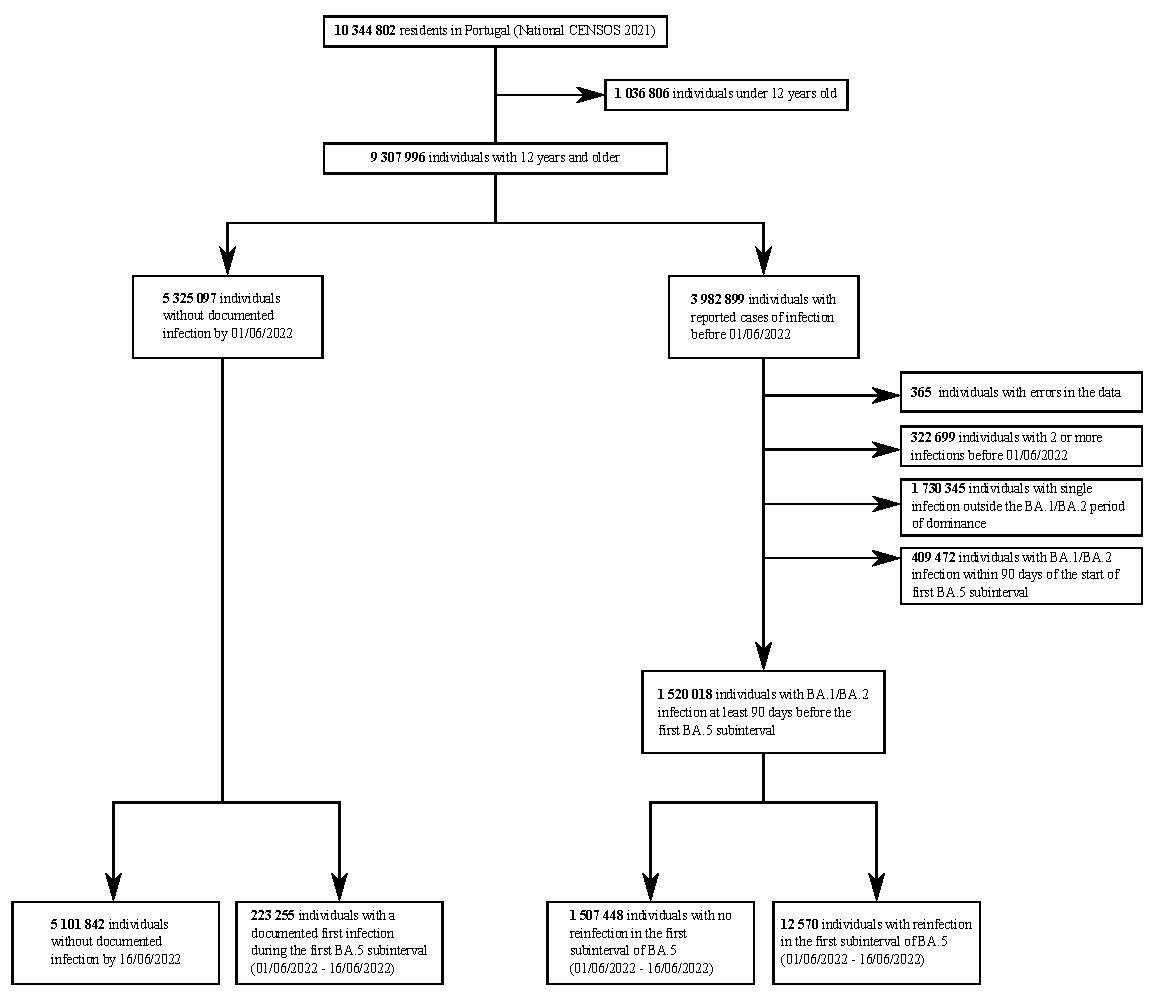
\includegraphics[width=0.91\linewidth]{chapter/2023-covid19-02/figures/ba5-1st-subvariant_risk_population-flow-chart_09.pdf}
    \caption[Flowchart describing the population selection]{Flowchart describing the population selection. Representative flowchart representing the selection for the first subinterval of BA.5 reinfection. For later BA.5 intervals, the 90-day period prior to the start of the interval allowed inclusion of a further subperiod of BA.1/BA.2 (Figure~\ref{fig:fig1-stability-hybrid-immunity}A). Note: the date format is day/month/year.}
    \label{fig:covid19-02-flowchart}
\end{figure}
% Figure 2
% Figure~\ref{fig:covid19-02-flowchart}

We used the national Covid-19 registry (SINAVE) to obtain information on all notified cases of infection, irrespective of clinical presentation. The ``uninfected'' population was defined as the population over 12 years of age without a documented infection in the registry at any time. The number of uninfected people on June 1st 2022 (the start of the BA.5 dominance period) was 5,325,097, representing 57\% of the Portuguese population over 12 (data from the National Census 20212).

The data available in SINAVE include cases of positive tests (PCR tests and rapid antigen tests) performed by healthcare workers in accredited diagnostic facilities. Testing by an accredited facility was a requisite for access to social security compensation for days of isolation---this is a reason for the comprehensiveness of the registry and the inclusion of only validated tests. Only tests performing above the EU-defined minimum for test sensitivity and specificity are used in Portugal. The testing policy officially changed on October 1st, 2022 but with some relaxation of the implementation in the period following their announcement just before the official date. Therefore, we considered infections until September 14th, 2022 as the period with consistent implementation of comprehensive testing policies.

We used the national SARS-CoV-2 genetic surveillance database \citep{institutonacionaldesaudedoutorricardojorge2022GeneticDiversity} to identify periods when one variant represented >90\% of the sample isolates, as also defined and used in other studies \citep{malatoRiskBAInfection2022, altarawneh2022ProtectiveEffect}. We assigned infected individuals to the variants' dominance periods and excluded all individuals who had more than one infection before the study period (Figure~\ref{fig:covid19-02-flowchart}). We pooled BA.1 and BA.2 infections, given the slow transition between the period of dominance of these two subvariants. With this approach, we identified the periods of dominance of BA.1/BA.2 (January 1st to April 17th, 2022) and of BA.5 infections (June 1st to September 14th, 2022). We then divided those periods of dominance into approximately 15 days intervals (as seen in Figure~\ref{fig:fig1-stability-hybrid-immunity}A). Coincidently, the period of BA.1/BA.2 dominance was divided into 7 sub-intervals, and the period of BA.5 was also divided into 7 sub-intervals (Table~\ref{tab:tabs1-variant-subinterval-periods} and Table~\ref{tab:tabs2-omicron-infection-risk}).

\begin{table}[h]
    \centering
    \caption[Subintervals of BA.1/BA.2 and BA.5 dominance used in the study]{Subintervals of BA.1/BA.2 and BA.5 dominance used in the study. Both periods of BA.1/BA.2 and BA.5 dominance were split in seven periods with approximately 2 weeks each. The fact that the two subvariants have the same number of intervals is a coincidence.}
    \begin{tblr}{
    hline{1,17} = {-}{0.08em},
    hline{2} = {-}{0.05em},
    column{1} = {l},
    column{2,3,4,5} = {c},
}
Variant  & Interval & Start date & End date & Days \\
BA1/BA.2 & A        & 01/01/22 & 16/01/22 & 15 \\
         & B        & 17/01/22 & 31/01/22 & 14 \\
         & C        & 01/02/22 & 15/02/22 & 14 \\
         & D        & 16/02/22 & 02/03/22 & 14 \\
         & E        & 03/03/22 & 18/03/22 & 15 \\
         & F        & 19/03/22 & 03/04/22 & 15 \\
         & G        & 04/04/22 & 17/04/22 & 13 \\
& & & & \\
BA.5     & a        & 01/06/22 & 16/06/22 & 15 \\
         & b        & 17/06/22 & 02/07/22 & 15 \\
         & c        & 03/07/22 & 16/07/22 & 13 \\
         & d        & 17/07/22 & 31/07/22 & 14 \\
         & e        & 01/08/22 & 14/08/22 & 13 \\
         & f        & 15/08/22 & 29/08/22 & 14 \\
         & g        & 30/08/22 & 14/09/22 & 15 
\end{tblr}
    % \resizebox{\textwidth}{!}{\begin{tblr}{
  row{1} = {m},
  column{1} = {l},
  column{2-7} = {c},
  hline{1,7} = {-}{0.08em},
  hline{2} = {-}{0.05em},
}
           & {Uninfected on\\June 1st} & {1st\\infection} & {BA.5\\infection} & {Absolute\\Risk} & RR (95\% CI)         & {Protection Efficacy, \%\\(95\% CI)} \\
Uninfected & 5 328 287                 & ---           & 367 783        & 0.069         & ---                  & ---                                  \\
Wuhan-Hu-1 & ---                       & 267 448       & 9 031          & 0.034         & 0.484 (0.474, 0.494) & 51.6 (50.6, 52.6)                    \\
Alpha      & ---                       & 20 004        & 647            & 0.032         & 0.452 (0.418, 0.489) & 54.8 (51.1, 58.2)                    \\
Delta      & ---                       & 232 831       & 6 329          & 0.027         & 0.387 (0.378, 0.397) & 61.3 (60.3, 62.2)                    \\
BA.1/BA.2  & ---                       & 1 557 635     & 22 793         & 0.015         & 0.247 (0.244, 0.250) & 75.3 (75.0, 75.6)                    
\end{tblr}}
    \label{tab:tabs1-variant-subinterval-periods}
\end{table}
% Table 1
% Table~\ref{tab:tabs1-variant-subinterval-periods}

\begin{table}
    \centering
    \caption[Risk of omicron BA.5 infection at different intervals for individuals infected with BA.1/BA.2 in specific periods]{Risk of omicron BA.5 infection at different intervals for individuals infected with BA.1/BA.2 in specific periods. We included in the study the population 12 years and older. Under ``1st infection'' is the number of individuals at risk for a second infection by BA.5 in the respective interval (i.e., without a second infection until that time). Note that the risk may depend on the epidemic situation and may differ in the BA.5 periods. RR, relative risk; CI, confidence interval.}
    % \resizebox{\textwidth}{10.5cm}{\begin{tblr}{
  column{even} = {c},
  column{1} = {r},
  column{2,3,4,5,6,7,8} = {c},
  hline{1,7,14,22,31,40,49,58} = {-}{0.08em},
  hline{2,8,15,23,32,41,50} = {-}{0.05em},
}
BA.5 (a) & Date interval & {Uninfected on\\Jun 1st 2022} & {1st\\infection} & {BA.5\\infection} & {Absolute\\risk} & {RR\\(95\% CI)} & {Protection efficacy, \%\\(95\% CI)}\\
 Uninfected &  & 5325097 & --- & 223255 & 0.042 & --- & ---\\
 BA.1/BA.2 A & 01/01/22--16/01/22 & --- & 421200 & 4130 & 0.010 & 0.240 (0.233, 0.248) & 75.97 (75.22, 76.68)\\
 B & 17/01/22--31/01/22 & --- & 620102 & 5488 & 0.009 & 0.223 (0.217, 0.229) & 77.69 (77.09, 78.26)\\
 C & 01/02/22--15/02/22 & --- & 341779 & 2328 & 0.007 & 0.165 (0.159, 0.172) & 83.46 (82.77, 84.11)\\
 D & 16/02/22--02/03/22 & --- & 136937 & 624 & 0.005 & 0.107 (0.099, 0.116) & 89.29 (88.41, 90.10)\\
BA.5 (b) & Date interval & {Uninfected on\\Jun 17th 2022} & {1st\\infection} & {BA.5\\infection} & {Absolute\\risk} & {RR\\(95\% CI)} & {Protection efficacy, \%\\(95\% CI)}\\
 Uninfected & --- & 5101842 & --- & 135093 & 0.026 & --- & ---\\
 BA.1/BA.2 A & 01/01/22--16/01/22 & --- & 417070 & 3004 & 0.007 & 0.283 (0.273, 0.293) & 71.73 (70.71, 72.72)\\
 B & 17/01/22--31/01/22 & --- & 614614 & 4103 & 0.007 & 0.269 (0.261, 0.278) & 73.07 (72.25, 73.87)\\
 C & 01/02/22--15/02/22 & --- & 339451 & 1803 & 0.005 & 0.207 (0.198, 0.217) & 79.31 (78.34, 80.24)\\
 D & 16/02/22--02/03/22 & --- & 136313 & 530 & 0.004 & 0.147 (0.135, 0.160) & 85.31 (84.01, 86.51)\\
 E & 03/03/22--18/03/22 & --- & 166811 & 356 & 0.002 & 0.081 (0.073, 0.090) & 91.89 (91.01, 92.69)\\
BA.5 (c) & Date interval & {Uninfected on\\Jul 3rd 2022} & {1st\\infection} & {BA.5\\infection} & {Absolute\\risk} & {RR\\(95\% CI)} & {Protection efficacy, \%\\(95\% CI)}\\
 Uninfected & --- & 4966749 & --- & 70757 & 0.014 & --- & ---\\
 BA.1/BA.2 A & 01/01/22--16/01/22 & --- & 414066 & 1616 & 0.004 & 0.287 (0.274, 0.302) & 71.26 (69.84, 72.62)\\
 B & 17/01/22--31/01/22 & --- & 610511 & 2295 & 0.004 & 0.284 (0.273, 0.296) & 71.57 (70.40, 72.69)\\
 C & 01/02/22--15/02/22 & --- & 337648 & 1140 & 0.003 & 0.247 (0.233, 0.261) & 75.34 (73.88, 76.73)\\
 D & 16/02/22--02/03/22 & --- & 135783 & 301 & 0.002 & 0.157 (0.141, 0.176) & 84.27 (82.39, 85.95)\\
 E & 03/03/22--18/03/22 & --- & 166455 & 249 & 0.001 & 0.107 (0.094, 0.121) & 89.32 (87.91, 90.57)\\
 F & 19/03/22--03/04/22 & --- & 133119 & 116 & 0.001 & 0.062 (0.052, 0.074) & 93.81 (92.58, 94.84)\\
BA.5 (d) & Date interval & {Uninfected on\\Jul 17th 2022} & {1st\\infection} & {BA.5\\infection} & {Absolute\\risk} & {RR\\(95\% CI)} & {Protection efficacy, \%\\(95\% CI)}\\
 Uninfected & --- & 4895992 & --- & 41767 & 0.009 & --- & ---\\
 BA.1/BA.2 A & 01/01/22--16/01/22 & --- & 412450 & 975 & 0.002 & 0.292 (0.274, 0.311) & 70.81 (68.94, 72.57)\\
 B & 17/01/22--31/01/22 & --- & 608216 & 1331 & 0.002 & 0.278 (0.264, 0.293) & 72.21 (70.70, 73.64)\\
 C & 01/02/22--15/02/22 & --- & 336508 & 701 & 0.002 & 0.255 (0.237, 0.275) & 74.49 (72.54, 76.30)\\
 D & 16/02/22--02/03/22 & --- & 135482 & 196 & 0.001 & 0.172 (0.150, 0.198) & 82.77 (80.19, 85.02)\\
 E & 03/03/22--18/03/22 & --- & 166206 & 191 & 0.001 & 0.138 (0.119, 0.159) & 86.23 (84.14, 88.05)\\
 F & 19/03/22--03/04/22 & --- & 133003 & 87 & 0.001 & 0.078 (0.063, 0.096) & 92.20 (90.38, 93.68)\\
 G & 04/04/22--17/04/22 & --- & 109542 & 61 & 0.001 & 0.066 (0.051, 0.085) & 93.39 (91.50, 94.85)\\
BA.5 (e) & Date interval & {Uninfected on\\Aug 1st 2022} & {1st\\infection} & {BA.5\\infection} & {Absolute\\risk} & {RR\\(95\% CI)} & {Protection efficacy, \%\\(95\% CI)}\\
 Uninfected & --- & 4854225 & --- & 28337 & 0.006 & --- & ---\\
 BA.1/BA.2 A & 01/01/22--16/01/22 & --- & 411475 & 657 & 0.002 & 0.289 (0.268, 0.312) & 71.12 (68.85, 73.22)\\
 B & 17/01/22--31/01/22 & --- & 606885 & 1000 & 0.002 & 0.306 (0.288, 0.325) & 69.44 (67.52, 71.25)\\
 C & 01/02/22--15/02/22 & --- & 335807 & 542 & 0.002 & 0.289 (0.266, 0.314) & 71.11 (68.59, 73.42)\\
 D & 16/02/22--02/03/22 & --- & 135286 & 161 & 0.001 & 0.207 (0.178, 0.242) & 79.26 (75.80, 82.22)\\
 E & 03/03/22--18/03/22 & --- & 166015 & 143 & 0.001 & 0.151 (0.128, 0.178) & 84.89 (82.20, 87.17)\\
 F & 19/03/22--03/04/22 & --- & 132916 & 79 & 0.001 & 0.104 (0.083, 0.129) & 89.62 (87.06, 91.67)\\
 G & 04/04/22--17/04/22 & --- & 109481 & 44 & 0.0004 & 0.070 (0.052, 0.094) & 93.01 (90.61, 94.80)\\
BA.5 (f) & Date interval & {Uninfected on\\Aug 15th 2022} & {1st\\infection} & {BA.5\\infection} & {Absolute\\risk} & {RR\\(95\% CI)} & {Protection efficacy, \%\\(95\% CI)}\\
 Uninfected & --- & 4825888 & --- & 29100 & 0.006 & --- & ---\\
 BA.1/BA.2 A & 01/01/22--16/01/22 & --- & 410818 & 660 & 0.002 & 0.282 (0.261, 0.304) & 71.85 (69.64, 73.89)\\
 B & 17/01/22--31/01/22 & --- & 605885 & 1011 & 0.002 & 0.300 (0.282, 0.319) & 70.02 (68.14, 71.78)\\
 C & 01/02/22--15/02/22 & --- & 335265 & 551 & 0.002 & 0.285 (0.262, 0.309) & 71.51 (69.05, 73.77)\\
 D & 16/02/22--02/03/22 & --- & 135125 & 198 & 0.001 & 0.247 (0.215, 0.284) & 75.30 (71.62, 78.50)\\
 E & 03/03/22--18/03/22 & --- & 165872 & 130 & 0.001 & 0.133 (0.112, 0.158) & 86.68 (84.19, 88.78)\\
 F & 19/03/22--03/04/22 & --- & 132837 & 83 & 0.001 & 0.106 (0.085, 0.131) & 89.44 (86.91, 91.48)\\
 G & 04/04/22--17/04/22 & --- & 109437 & 57 & 0.001 & 0.088 (0.068, 0.114) & 91.23 (88.63, 93.23)\\
BA.5 (g) & Date interval & {Uninfected on\\Aug 30th 2022} & {1st\\infection} & {BA.5\\infection} & {Absolute\\risk} & {RR\\(95\% CI)} & {Protection efficacy, \%\\(95\% CI)}\\
 Uninfected & --- & 4796788 & --- & 28125 & 0.006 & --- & ---\\
 BA.1/BA.2 A & 01/01/22--16/01/22 & --- & 410158 & 738 & 0.002 & 0.323 (0.301, 0.347) & 67.66 (65.27, 69.89)\\
 B & 17/01/22--31/01/22 & --- & 604874 & 1290 & 0.002 & 0.390 (0.370, 0.412) & 60.97 (58.82, 63.00)\\
 C & 01/02/22--15/02/22 & --- & 334714 & 685 & 0.002 & 0.363 (0.337, 0.391) & 63.68 (60.89, 66.27)\\
 D & 16/02/22--02/03/22 & --- & 134927 & 235 & 0.002 & 0.302 (0.266, 0.343) & 69.83 (65.73, 73.44)\\
 E & 03/03/22--18/03/22 & --- & 165742 & 193 & 0.001 & 0.203 (0.176, 0.234) & 79.69 (76.62, 82.35)\\
 F & 19/03/22--03/04/22 & --- & 132754 & 108 & 0.001 & 0.141 (0.117, 0.171) & 85.87 (82.94, 88.29)\\
 G & 04/04/22--17/04/22 & --- & 109380 & 72 & 0.001 & 0.114 (0.090, 0.144) & 88.60 (85.65, 90.95)
\end{tblr}}
    \resizebox*{0.9\textwidth}{\dimexpr\textheight-2\baselineskip\relax}{\begin{tblr}{
  column{even} = {c},
  column{1} = {r},
  column{2,3,4,5,6,7,8} = {c},
  hline{1,7,14,22,31,40,49,58} = {-}{0.08em},
  hline{2,8,15,23,32,41,50} = {-}{0.05em},
}
BA.5 (a) & Date interval & {Uninfected on\\Jun 1st 2022} & {1st\\infection} & {BA.5\\infection} & {Absolute\\risk} & {RR\\(95\% CI)} & {Protection efficacy, \%\\(95\% CI)}\\
 Uninfected &  & 5325097 & --- & 223255 & 0.042 & --- & ---\\
 BA.1/BA.2 A & 01/01/22--16/01/22 & --- & 421200 & 4130 & 0.010 & 0.240 (0.233, 0.248) & 75.97 (75.22, 76.68)\\
 B & 17/01/22--31/01/22 & --- & 620102 & 5488 & 0.009 & 0.223 (0.217, 0.229) & 77.69 (77.09, 78.26)\\
 C & 01/02/22--15/02/22 & --- & 341779 & 2328 & 0.007 & 0.165 (0.159, 0.172) & 83.46 (82.77, 84.11)\\
 D & 16/02/22--02/03/22 & --- & 136937 & 624 & 0.005 & 0.107 (0.099, 0.116) & 89.29 (88.41, 90.10)\\
BA.5 (b) & Date interval & {Uninfected on\\Jun 17th 2022} & {1st\\infection} & {BA.5\\infection} & {Absolute\\risk} & {RR\\(95\% CI)} & {Protection efficacy, \%\\(95\% CI)}\\
 Uninfected & --- & 5101842 & --- & 135093 & 0.026 & --- & ---\\
 BA.1/BA.2 A & 01/01/22--16/01/22 & --- & 417070 & 3004 & 0.007 & 0.283 (0.273, 0.293) & 71.73 (70.71, 72.72)\\
 B & 17/01/22--31/01/22 & --- & 614614 & 4103 & 0.007 & 0.269 (0.261, 0.278) & 73.07 (72.25, 73.87)\\
 C & 01/02/22--15/02/22 & --- & 339451 & 1803 & 0.005 & 0.207 (0.198, 0.217) & 79.31 (78.34, 80.24)\\
 D & 16/02/22--02/03/22 & --- & 136313 & 530 & 0.004 & 0.147 (0.135, 0.160) & 85.31 (84.01, 86.51)\\
 E & 03/03/22--18/03/22 & --- & 166811 & 356 & 0.002 & 0.081 (0.073, 0.090) & 91.89 (91.01, 92.69)\\
BA.5 (c) & Date interval & {Uninfected on\\Jul 3rd 2022} & {1st\\infection} & {BA.5\\infection} & {Absolute\\risk} & {RR\\(95\% CI)} & {Protection efficacy, \%\\(95\% CI)}\\
 Uninfected & --- & 4966749 & --- & 70757 & 0.014 & --- & ---\\
 BA.1/BA.2 A & 01/01/22--16/01/22 & --- & 414066 & 1616 & 0.004 & 0.287 (0.274, 0.302) & 71.26 (69.84, 72.62)\\
 B & 17/01/22--31/01/22 & --- & 610511 & 2295 & 0.004 & 0.284 (0.273, 0.296) & 71.57 (70.40, 72.69)\\
 C & 01/02/22--15/02/22 & --- & 337648 & 1140 & 0.003 & 0.247 (0.233, 0.261) & 75.34 (73.88, 76.73)\\
 D & 16/02/22--02/03/22 & --- & 135783 & 301 & 0.002 & 0.157 (0.141, 0.176) & 84.27 (82.39, 85.95)\\
 E & 03/03/22--18/03/22 & --- & 166455 & 249 & 0.001 & 0.107 (0.094, 0.121) & 89.32 (87.91, 90.57)\\
 F & 19/03/22--03/04/22 & --- & 133119 & 116 & 0.001 & 0.062 (0.052, 0.074) & 93.81 (92.58, 94.84)\\
BA.5 (d) & Date interval & {Uninfected on\\Jul 17th 2022} & {1st\\infection} & {BA.5\\infection} & {Absolute\\risk} & {RR\\(95\% CI)} & {Protection efficacy, \%\\(95\% CI)}\\
 Uninfected & --- & 4895992 & --- & 41767 & 0.009 & --- & ---\\
 BA.1/BA.2 A & 01/01/22--16/01/22 & --- & 412450 & 975 & 0.002 & 0.292 (0.274, 0.311) & 70.81 (68.94, 72.57)\\
 B & 17/01/22--31/01/22 & --- & 608216 & 1331 & 0.002 & 0.278 (0.264, 0.293) & 72.21 (70.70, 73.64)\\
 C & 01/02/22--15/02/22 & --- & 336508 & 701 & 0.002 & 0.255 (0.237, 0.275) & 74.49 (72.54, 76.30)\\
 D & 16/02/22--02/03/22 & --- & 135482 & 196 & 0.001 & 0.172 (0.150, 0.198) & 82.77 (80.19, 85.02)\\
 E & 03/03/22--18/03/22 & --- & 166206 & 191 & 0.001 & 0.138 (0.119, 0.159) & 86.23 (84.14, 88.05)\\
 F & 19/03/22--03/04/22 & --- & 133003 & 87 & 0.001 & 0.078 (0.063, 0.096) & 92.20 (90.38, 93.68)\\
 G & 04/04/22--17/04/22 & --- & 109542 & 61 & 0.001 & 0.066 (0.051, 0.085) & 93.39 (91.50, 94.85)\\
BA.5 (e) & Date interval & {Uninfected on\\Aug 1st 2022} & {1st\\infection} & {BA.5\\infection} & {Absolute\\risk} & {RR\\(95\% CI)} & {Protection efficacy, \%\\(95\% CI)}\\
 Uninfected & --- & 4854225 & --- & 28337 & 0.006 & --- & ---\\
 BA.1/BA.2 A & 01/01/22--16/01/22 & --- & 411475 & 657 & 0.002 & 0.289 (0.268, 0.312) & 71.12 (68.85, 73.22)\\
 B & 17/01/22--31/01/22 & --- & 606885 & 1000 & 0.002 & 0.306 (0.288, 0.325) & 69.44 (67.52, 71.25)\\
 C & 01/02/22--15/02/22 & --- & 335807 & 542 & 0.002 & 0.289 (0.266, 0.314) & 71.11 (68.59, 73.42)\\
 D & 16/02/22--02/03/22 & --- & 135286 & 161 & 0.001 & 0.207 (0.178, 0.242) & 79.26 (75.80, 82.22)\\
 E & 03/03/22--18/03/22 & --- & 166015 & 143 & 0.001 & 0.151 (0.128, 0.178) & 84.89 (82.20, 87.17)\\
 F & 19/03/22--03/04/22 & --- & 132916 & 79 & 0.001 & 0.104 (0.083, 0.129) & 89.62 (87.06, 91.67)\\
 G & 04/04/22--17/04/22 & --- & 109481 & 44 & 0.0004 & 0.070 (0.052, 0.094) & 93.01 (90.61, 94.80)\\
BA.5 (f) & Date interval & {Uninfected on\\Aug 15th 2022} & {1st\\infection} & {BA.5\\infection} & {Absolute\\risk} & {RR\\(95\% CI)} & {Protection efficacy, \%\\(95\% CI)}\\
 Uninfected & --- & 4825888 & --- & 29100 & 0.006 & --- & ---\\
 BA.1/BA.2 A & 01/01/22--16/01/22 & --- & 410818 & 660 & 0.002 & 0.282 (0.261, 0.304) & 71.85 (69.64, 73.89)\\
 B & 17/01/22--31/01/22 & --- & 605885 & 1011 & 0.002 & 0.300 (0.282, 0.319) & 70.02 (68.14, 71.78)\\
 C & 01/02/22--15/02/22 & --- & 335265 & 551 & 0.002 & 0.285 (0.262, 0.309) & 71.51 (69.05, 73.77)\\
 D & 16/02/22--02/03/22 & --- & 135125 & 198 & 0.001 & 0.247 (0.215, 0.284) & 75.30 (71.62, 78.50)\\
 E & 03/03/22--18/03/22 & --- & 165872 & 130 & 0.001 & 0.133 (0.112, 0.158) & 86.68 (84.19, 88.78)\\
 F & 19/03/22--03/04/22 & --- & 132837 & 83 & 0.001 & 0.106 (0.085, 0.131) & 89.44 (86.91, 91.48)\\
 G & 04/04/22--17/04/22 & --- & 109437 & 57 & 0.001 & 0.088 (0.068, 0.114) & 91.23 (88.63, 93.23)\\
BA.5 (g) & Date interval & {Uninfected on\\Aug 30th 2022} & {1st\\infection} & {BA.5\\infection} & {Absolute\\risk} & {RR\\(95\% CI)} & {Protection efficacy, \%\\(95\% CI)}\\
 Uninfected & --- & 4796788 & --- & 28125 & 0.006 & --- & ---\\
 BA.1/BA.2 A & 01/01/22--16/01/22 & --- & 410158 & 738 & 0.002 & 0.323 (0.301, 0.347) & 67.66 (65.27, 69.89)\\
 B & 17/01/22--31/01/22 & --- & 604874 & 1290 & 0.002 & 0.390 (0.370, 0.412) & 60.97 (58.82, 63.00)\\
 C & 01/02/22--15/02/22 & --- & 334714 & 685 & 0.002 & 0.363 (0.337, 0.391) & 63.68 (60.89, 66.27)\\
 D & 16/02/22--02/03/22 & --- & 134927 & 235 & 0.002 & 0.302 (0.266, 0.343) & 69.83 (65.73, 73.44)\\
 E & 03/03/22--18/03/22 & --- & 165742 & 193 & 0.001 & 0.203 (0.176, 0.234) & 79.69 (76.62, 82.35)\\
 F & 19/03/22--03/04/22 & --- & 132754 & 108 & 0.001 & 0.141 (0.117, 0.171) & 85.87 (82.94, 88.29)\\
 G & 04/04/22--17/04/22 & --- & 109380 & 72 & 0.001 & 0.114 (0.090, 0.144) & 88.60 (85.65, 90.95)
\end{tblr}}
    \label{tab:tabs2-omicron-infection-risk}
\end{table}
% Table 2
% Table~\ref{tab:tabs2-omicron-infection-risk}

Reinfection was defined as two positive tests in the same individual, at least 90 days apart \citep{worldhealthorganizaton2022PublicHealth}. Consequently, all cases of infection in the 90 days before the start of each sub-interval were not included, as these would not classify as ``at risk of reinfection'' for the entire duration of the subinterval under the definition above.

Given the high vaccine coverage, we compared one population with ``hybrid immunity'' (vaccination $+$ infection with BA.1/BA.2) with a group of vaccinated individuals without infection. In other words, we assessed the stability of hybrid immunity (induced with Omicron BA.1/BA.2 infection $+$ vaccines) versus vaccine immunity. The change in the relative risk that we report, translates the waning of such ``additional'' protection afforded by natural infection of the vaccinated individuals.

It is possible that the population we classified as ``uninfected'' contains individuals with a prior unnoticed infection (i.e., asymptomatic infection). In a previous publication, we have shown that considering a proportion (20\%--40\%) of unreported infections within the ``uninfected'' group (in line with data from the national serologic survey \citep{institutonacionaldesaudedoutorricardojorge2021NationalCOVID19}) only has the effect of decreasing slightly the relative risk of BA.5 re-infection in each sub-interval \citep{malatoRiskBAInfection2022}, without changing our overall results. This is intuitive because if more people were infected (and moved out of the ``uninfected group''), that inflates the absolute risk of first infection, and thus the relative risk of a second infection with BA.5 decreases. 

In conclusion, the study design is similar to a prospective study but taking place in the past: the groups of interest were selected (i.e., individuals with no recorded infection or individuals with one infection in a defined period of time and without any additional infection reported until the start of the study period); and afterwards the individuals from the different groups were followed, under the same epidemiological conditions, for a pre-defined (and equal) number of days and their infections were recorded. We considered other study designs, such as test-negative study \citep{altarawneh2022ProtectiveEffect, ayoub2022EstimatingProtection, hansen2023RiskReinfection}, but our registry-based dataset only includes information on positive tests, thus precluding the use of a test-negative design.

%%%%%%%%%%%%%%%%%%%%%%%%%%%%%%%%%%%%%%%%%%%%%%%%%%%%%%%%%%%%%%%%%%%%%%%%
\subsection{Vaccination coverage}

The vaccine coverage with the primary vaccination series in the Portuguese residents over 12 years was >98\% by the end of 2021. The primary series of the vaccination campaign used EU/EMA-authorized vaccines: Comirnaty (Pfizer/BioNTech), 69\%; Spikevax (Moderna), 12\%; Vaxzevria (AstraZeneca), 13\%; and Janssen 6\%.

While at the start of the BA.1/BA.2 period of dominance (January 1st, 2022), the coverage with the first booster was residual (mostly long-term care facility residents), at the start of the BA.5 period of dominance (June 1st), the coverage with the first booster was 82\%. The vaccine boosters relied exclusively on mRNA vaccines (77\% Comirnaty and 23\% Spikevax). At the start of the BA.5 period, a second booster was not yet in use except for a highly specific (and very small) population of patients with severe immunosuppression.

%%%%%%%%%%%%%%%%%%%%%%%%%%%%%%%%%%%%%%%%%%%%%%%%%%%%%%%%%%%%%%%%%%%%%%%%
\subsection{Statistical analysis}

We estimated the relative risk of BA.5 reinfection in each sub-interval using the modified Poisson regression method with a robust sandwich estimator for the variance as described previously \citep{zou2004ModifiedPoisson}. We compared the risk of BA.5 infection for people with a previous single infection at different intervals, with the same risk for people without any previously recorded infection in the same interval periods (Table~\ref{tab:tabs2-omicron-infection-risk}). Protection efficacy was estimated, in percentage, as $(1 - \text{RR}) \times 100\%$. Confidence intervals for the RR were calculated using the Wald normal approximation method, with the epitools R package \citep{aragon2020EpitoolsEpidemiology}.

To ascertain the change in relative risk over time, we considered the sub-intervals of BA.5 infection as a blocking factor and used a mixed-effect approach to estimate the change in risk over time, where ``sub-interval'' was the random effect \citep{pinheiro2000MixedEffectsModels}. We fitted the increase in risk with the following saturating function:
% 
\begin{equation}
    \text{RR}(t \geq 90) = rr_0 + (rr_A - rr_0) \frac{(t-90)^n}{T_M^n + (t-90)^n}\ .
    \label{eq:omicron-infection-risk}
\end{equation}
% Equation (1)
% Equation~(\ref{eq:omicron-infection-risk})

In this equation, $t$ represents time in days, which is larger than 90, since re-infections can only occur after that time, $rr_0$ is the initial relative risk when $t = 90$, and $rr_A$ is the asymptotic risk when time is very large, $T_M$ is the time, after 90 days, at which the relative risk is approximately \(\frac{1}{2}\) of the asymptotic risk. Finally, $n$ allows for different steepness in the increase of relative risk. This is a general saturation function, and it allowed us to test simpler versions, such as fixing $rr_A = 1$ or $n = 1$, which did not describe the data as well. We also tested other saturation functions, such as logistic or generalised logistics, but the results were similar (i.e., the initial and the asymptotic relative risk). We used the software Monolix 2021R1 (Lixoft SAS, Antony, France) to fit this model using each sub-interval of BA.5 as the random effect (Figure~\ref{fig:fig1-stability-hybrid-immunity}B and Figure~\ref{fig:figs2-rr-variation-to-ba5}). The best fit included a random effect for $T_M$ and $n$, but only fixed effects for $rr_0$ and $rr_A$. The population parameters for the best mixed-effect fit are $rr_0 = 0.064$ (95\% CI = [0.056, 0.074]), $rr_A = 0.368$ (95\% CI = [0.321, 0.424]), $T_M = 65.7$ (95\% CI = [52.8, 81.9]), $n = 3.2$ (95\% CI = [2.3, 4.4]). The stability of the estimated parameters for initial and asymptotic relative risk (with no random effect supported by the data) over the different time intervals strengthens our conclusions, as biases due to, for example, undocumented infections are unlikely to be important for the periods studied.

\begin{figure}[h]
    \centering
    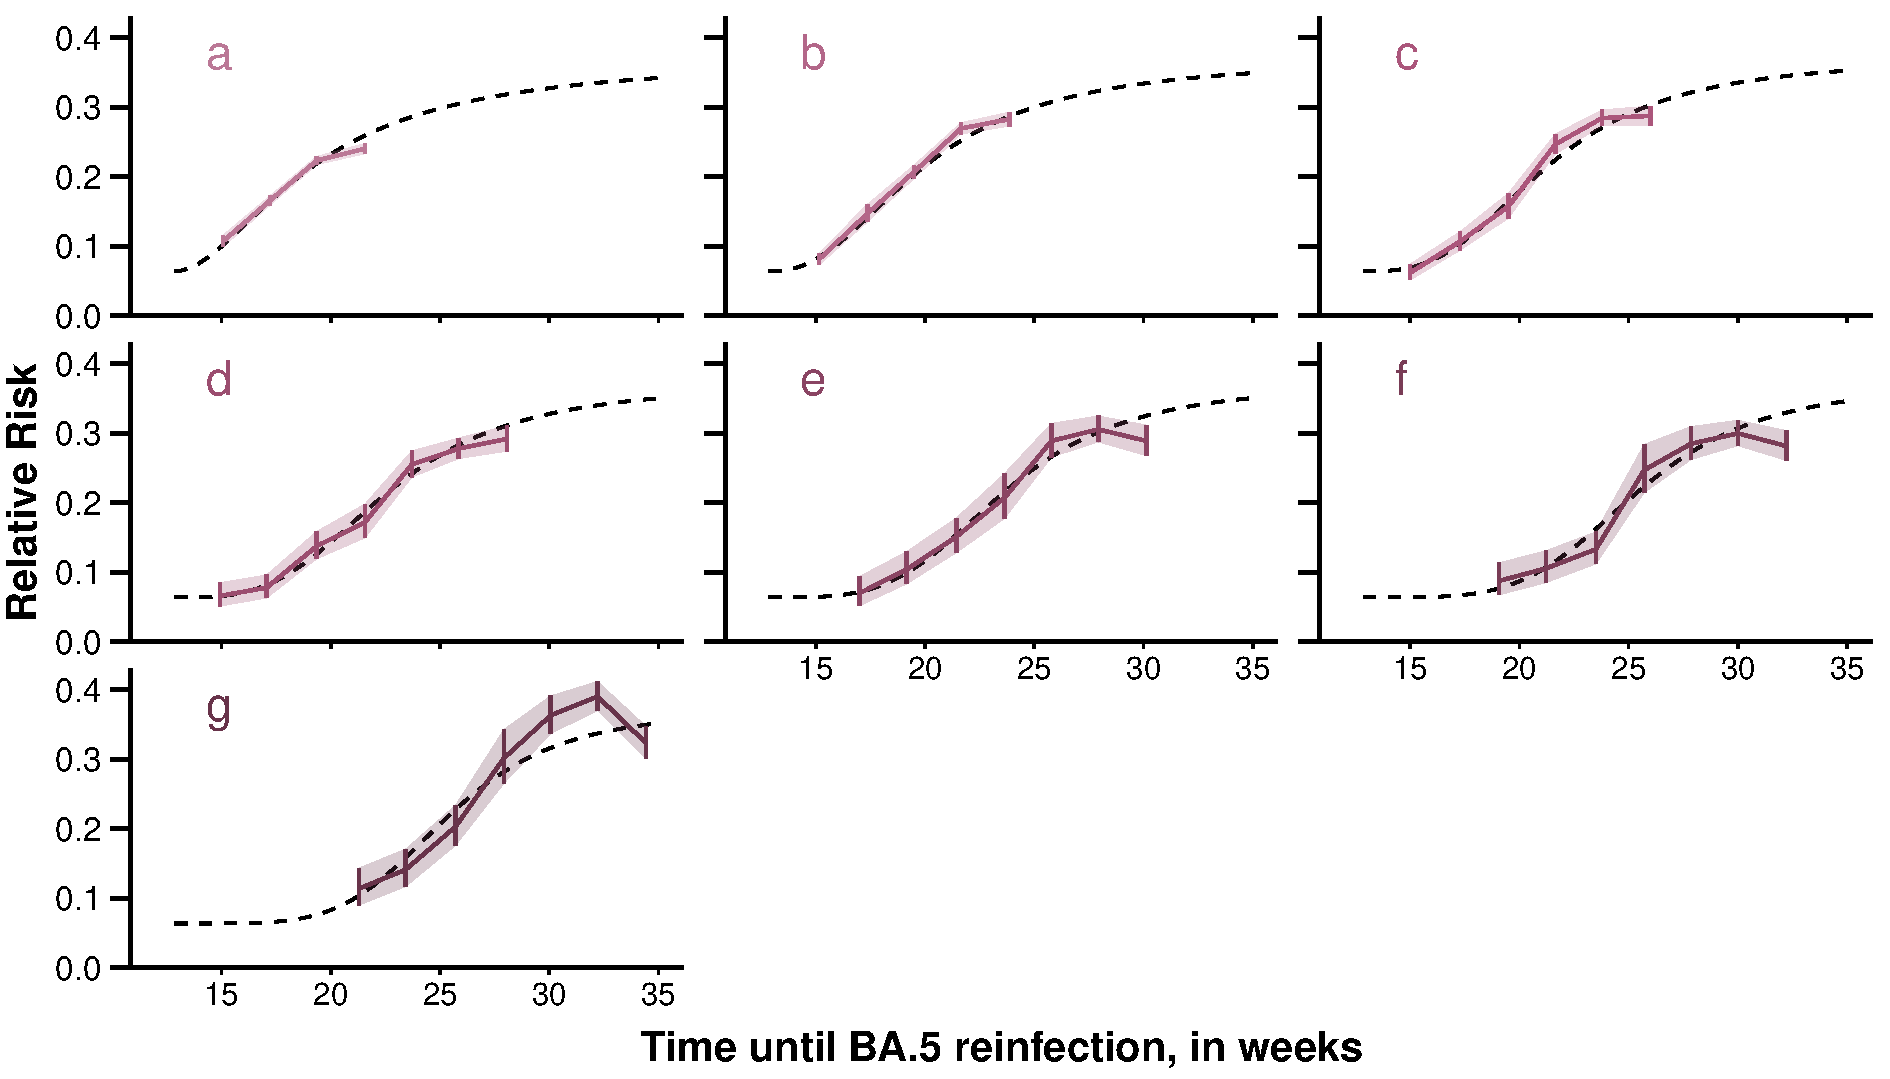
\includegraphics[width=0.9\textwidth]{chapter/2023-covid19-02/figures/2022-11-07_figure-s2-v1.pdf}
    \caption[Variation of RR of protection against BA.5 infection over time since BA.1/BA.2 infection]{Variation of RR of protection against BA.5 infection over time since BA.1/BA.2 infection. Individual sub-interval fits of Equation~(\ref{eq:omicron-infection-risk}) (dashed lines) to the different periods of BA.5 dominance (intervals a to g), corresponding to the population fit presented in Figure~\ref{fig:fig1-stability-hybrid-immunity}B. The RR calculated from the data is indicated in the solid lines with corresponding 95\% confidence intervals (shaded area).}
    \label{fig:figs2-rr-variation-to-ba5}
\end{figure}
% Figure 3
% Figure~\ref{fig:figs2-rr-variation-to-ba5}

% \vfill
% \newpage

\clearpage
%%%%%%%%%%%%%%%%%%%%%%%%%%%%%%%%%%%%%%%%%%%%%%%%%%%%%%%%%%%%%%%%%%%%%%%%
\addcontentsline{toc}{section}{Bibliography}
\bibliographystyle{abbrvnat}
\bibliography{references}
%%%%%%%%%%%%%%%%%%%%%%%%%%%%%%%%%%%%%%%%%%%%%%%%%%%%%%%%%%%%%%%%%%%%%%%%

% Table 1
% Table~\ref{tab:tabs1-variant-subinterval-periods}
% Table 2
% Table~\ref{tab:tabs2-omicron-infection-risk}

% Figure 1
% Figure~\ref{fig:fig1-stability-hybrid-immunity}
% Figure 2
% Figure~\ref{fig:covid19-02-flowchart}
% Figure 3
% Figure~\ref{fig:figs2-rr-variation-to-ba5}

% Equation (1)
% Equation~(\ref{eq:omicron-infection-risk})